\documentclass[tikz]{standalone}
\usetikzlibrary{automata,positioning}
\begin{document}

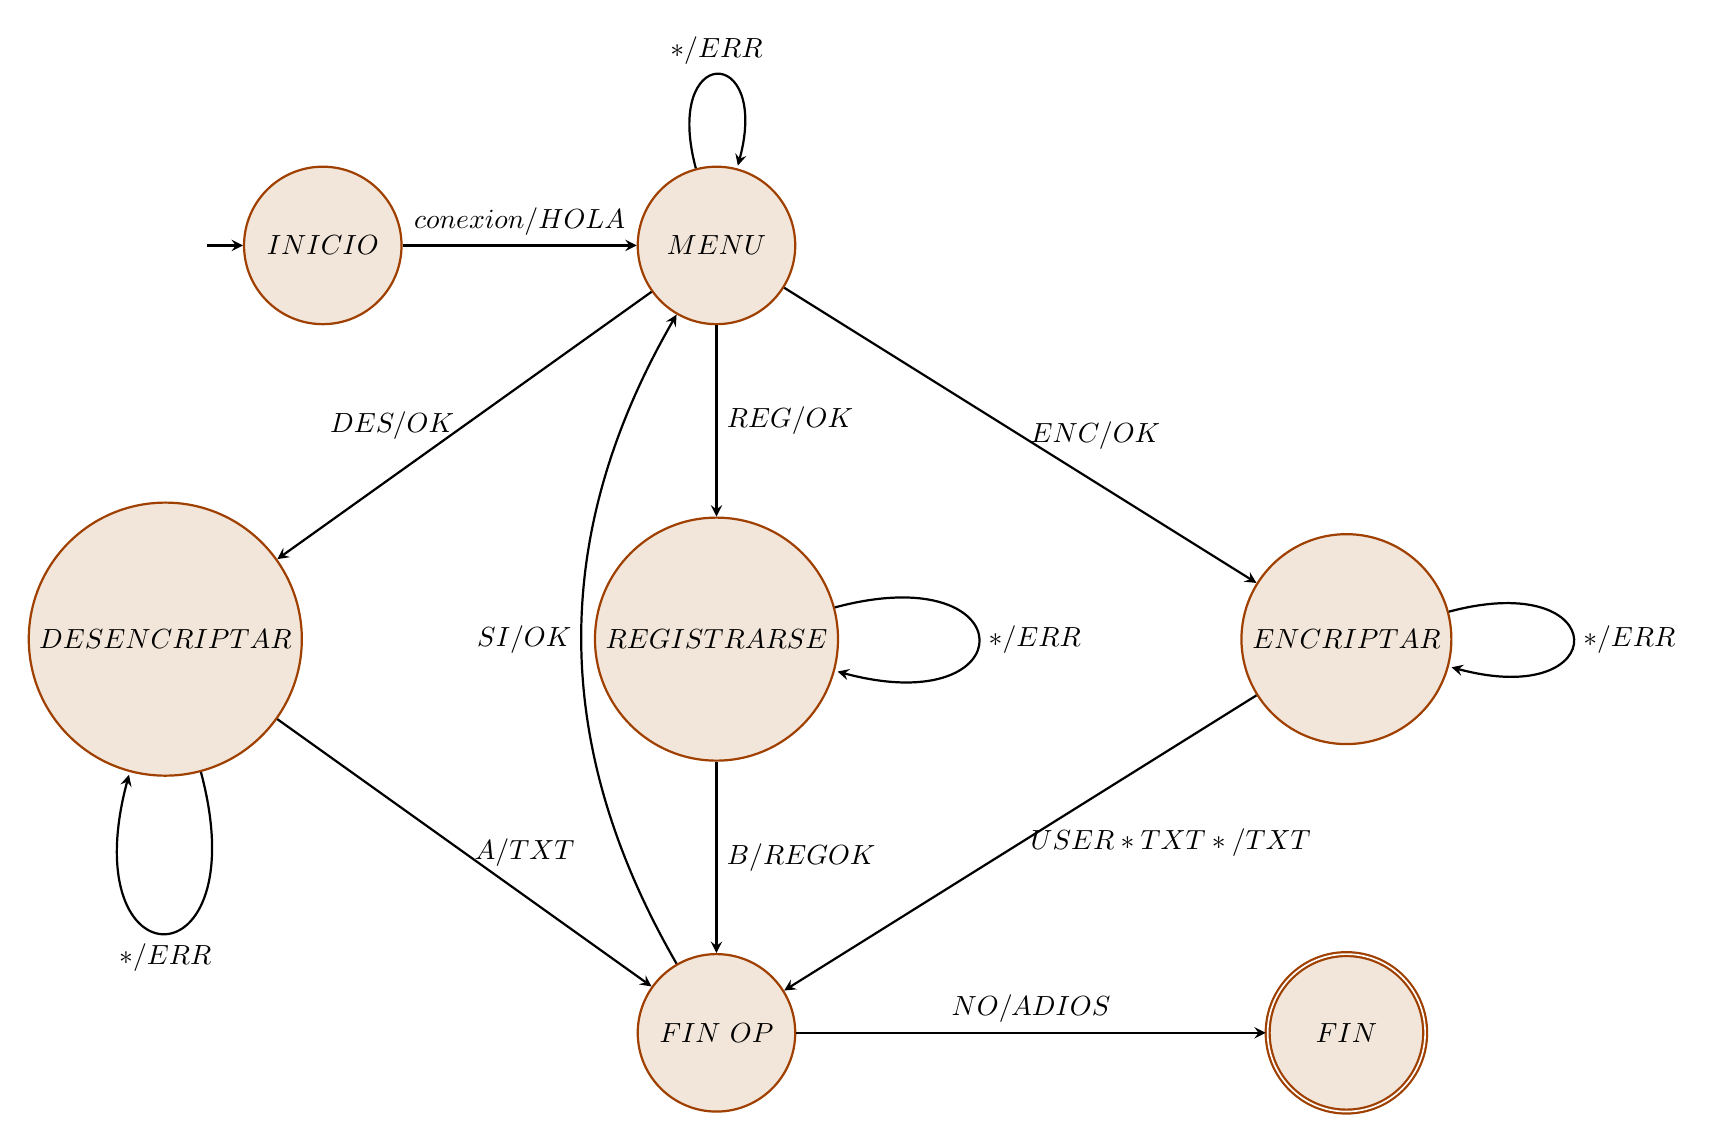
\begin{tikzpicture}[>=stealth,node distance=3cm,on grid, auto, thick, initial text=]
	\tikzstyle{state}=[circle,thick,draw=brown!150,fill=brown!20,minimum size=20mm]

	\node[state,initial] 	(INICIO)	{$INICIO$};
	\node[state] (MENU) [right=5cm of INICIO] {$MENU$};
	\node[state] (SINGUP)	[below=5cm of MENU] {$REGISTRARSE$};
	\node[state] (DESENCRIPTAR) [left=7cm of SINGUP] {$DESENCRIPTAR$};
	\node[state] (ENCRIPTAR) [right=8cm of SINGUP] {$ENCRIPTAR$};
	\node[state] (FIN_OP)		[below=5cm of SINGUP] {$FIN\ OP$};
	\node[state,accepting] (FIN) [right=8cm of FIN_OP] {$FIN$};
	
	\path[->]	(INICIO) edge node[above] {$conexion/HOLA$} (MENU)
				(MENU) edge [loop above] node[above] {$*/ERR$} (MENU)
				(MENU) edge node[left] {$DES/ OK$} (DESENCRIPTAR)
				(DESENCRIPTAR) edge [loop below] node[below] {$*/ERR$} (DESENCRIPTAR)
				(MENU) edge node[right] {$ENC/OK$} (ENCRIPTAR)
				(ENCRIPTAR) edge [loop right] node[right] {$*/ERR$} (ENCRIPTAR)
				(MENU) edge node[right] {$REG/OK$} (SINGUP)
				(SINGUP) edge [loop right] node[right] {$*/ERR$} (SINGUP)
				(ENCRIPTAR) edge node[right] {$USER*TXT*/TXT$} (FIN_OP)
				(DESENCRIPTAR) edge node[right] {$A/TXT$} (FIN_OP)
				(SINGUP) edge node[right] {$B/REGOK$} (FIN_OP)
				(FIN_OP) edge [bend left] node[left] {$SI/OK$} (MENU)
				(FIN_OP) edge node[above] {$NO/ADIOS$} (FIN);
					
		
\end{tikzpicture}
\end{document}
